\documentclass{xdupgthesis}
\usepackage{amsmath}
\usepackage{amssymb}
\usepackage{longtable}
\usepackage{subcaption}

\xdusetup{
    style = { 
        cjk-font = fandol, 
        latin-font = gyre,
        biblatex-option = {doi=false, url = false},
        % 信息移除
        % remove-page = { 致谢 }, 
        % anonymous = true,
        % 对照表
        customize-los = false,
        colspec-los   = {>{\hskip1cm}Q[l,h]<{\hskip2cm}X[l,h]},
        customize-loa = false,
        colspec-loa   = {>{\hskip1cm}Q[l,h]<{\hskip1cm}X[-1,l,h]X[-1,l,h]} 
    },
    info = {
        author = {李明一},
        author* = {Mingyi Li},
        student-id = {xx15xxxxxxx},
        department = {计算机科学学院},
        major = {计算机科学},
        major* = {Computer Science},
        sub-major = {人工智能},
        graduate-type = {硕士},
        degree = {工学硕士},
        % degree* = {},
        degree-type = {学术},
        bio = {res/profile.tex},
        supervisor = {张伟}, 
        supervisor* = {Wei Zhang}, 
        supv-title = {副教授},
        supv-title* = {Associate Professor},
        title = {单一文件如何层次拆分出规范工程的研究},
        title* = {Research on How to Decompose a Single File into Normative Engineering Hierarchically},
        clc = {TN82},
        secret-level = {公开},
        submit-date = {2025-05-01},
        abstract = {chapters/abstract-zh.tex},
        keywords = {关键词},
        keywords* = {keyword},
        abstract* = {chapters/abstract-en.tex},
        acknowledgements = {chapters/acknowledgements.tex},
        bib-resource = {reference.bib},
        statement-scan = {},
        statement-sign = {},
        %符号对照表
        los = {res/notion.tex},
        %缩略语对照表
        loa = {res/loa.tex},
        %附录
        appendix = {res/appendix.tex},
    }
}

\begin{document}

\chapter{绪论}
引用参考文献~\cite{pipl2021}

\section{研究背景及意义}

\section{研究历史与现状}

\subsection{分类方向1}

\subsection{分类方向2}

\subsection{分类方向3}

\subsection{分类方向4}

\section{本论文组织结构}
本文的组织结构安排如下:
第一章为绪论,主要介绍了...

第二章主要介绍...


\chapter{相关知识技术}
\section{引言}

\section{xx基础}

\subsection{xx网络}

\subsection{xx函数}

\section{xx基础}
\subsection{xx网络}

\subsection{xx函数}

\section{本章小结}
本章节首先介绍了xx基础...

\chapter{xx技术}
\label{chapter:work1}
\section{引言}
\section{xx机制}
\subsection{符号与定义}
\subsection{xx设计}
\subsection{xx实现流程}
\subsection{总结与扩展}

\section{实验与性能评估}
\subsection{实验设置}
\subsection{性能概述}
\subsection{超参数分析}

\section{本章小结}



\chapter{xx技术}
\label{chapter:work2}
\section{引言}
\section{xx机制}
总框架:~\ref{fig:arch}

\begin{figure}[!ht]
\centering
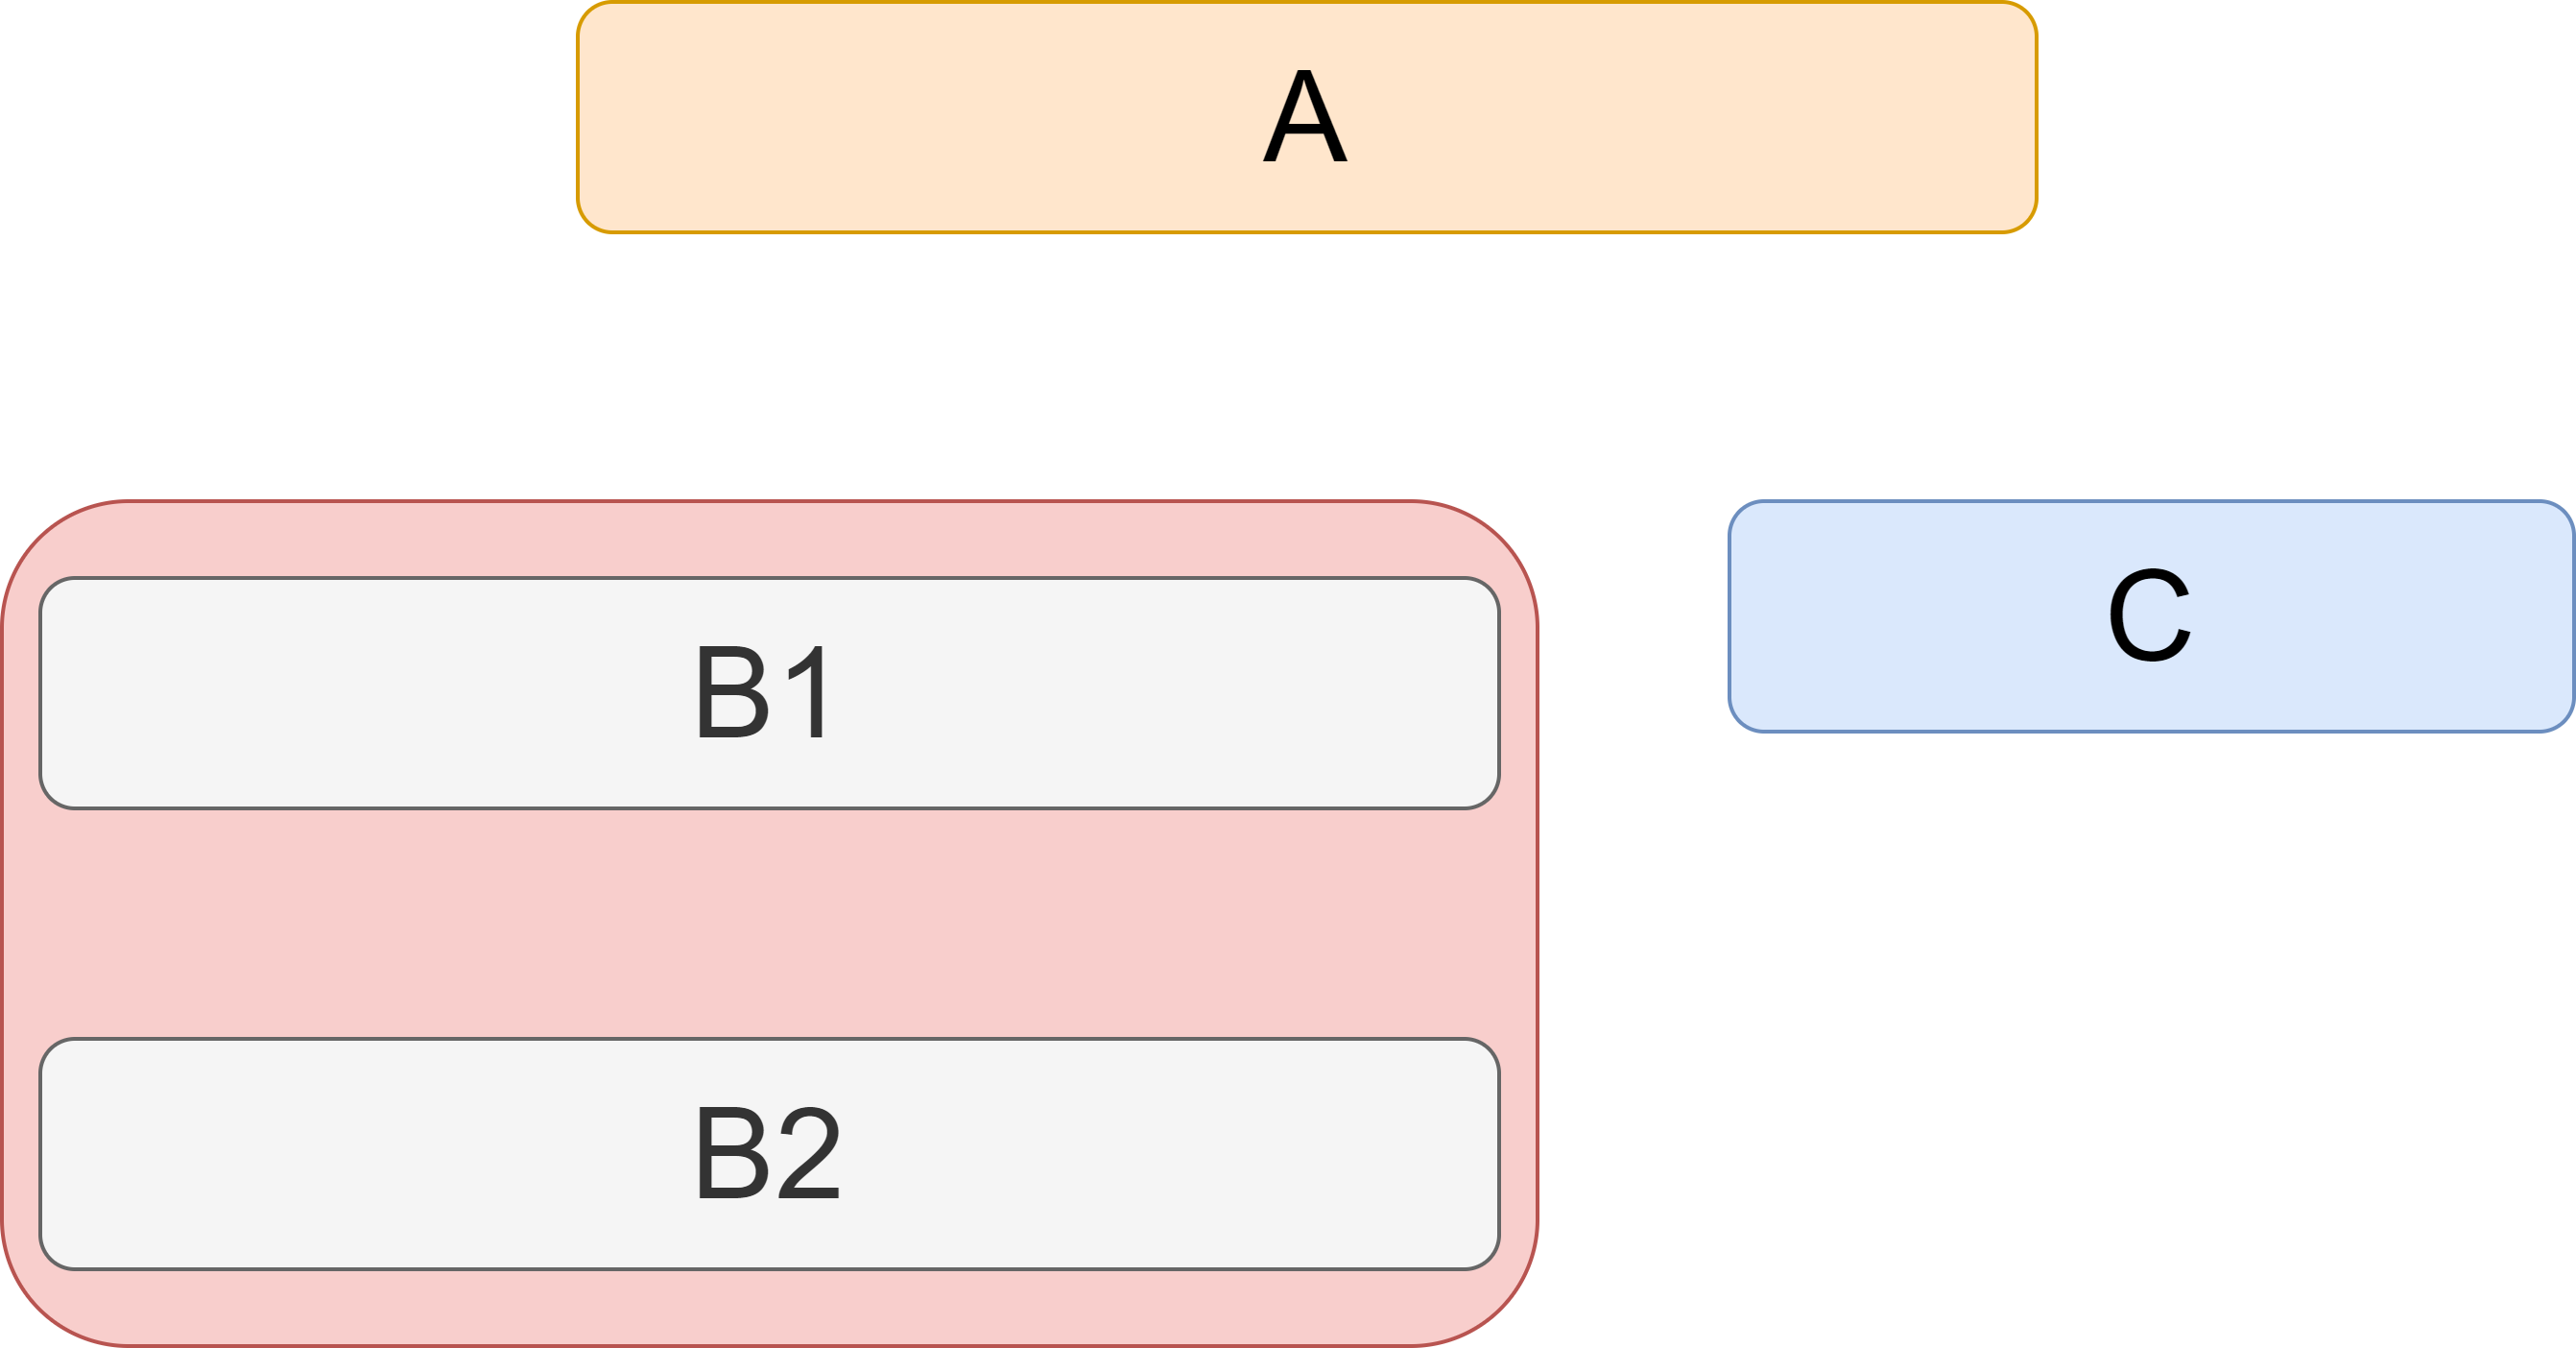
\includegraphics[width=\textwidth]{res/figs/arch.png}
\caption{工作架构图}
\label{fig:arch}
\end{figure}

\section{实验与性能评估}

\section{本章小结}



\chapter{总结与展望}
\section{全文总结}
\section{后续工作展望}



\end{document}
